\documentclass[12pt]{article}

\usepackage[english]{babel}
\usepackage[utf8x]{inputenc}
\usepackage{graphicx}
\linespread{1}
%\pagestyle{empty}
\setlength\parindent{12pt}


\usepackage[top=1in,bottom=1in,left=1in,right=1in]{geometry}
\title{Decentralized Approaches for Autonomous Intersection Control }
\author{Ariel Anders and Noel Hollingsworth\\ 6.852 Final Project Type: Reading Project}

\begin{document}
\maketitle 

\pagebreak
\tableofcontents
\pagebreak

\section{Introduction}

Traffic congestion is one of the leading causes of lost productivity and decreased standard of living in urban settings. Recent advances in artificial intelligence suggest vehicle navigation by autonomous agents will be possible in the near future.\cite{dresner}  
% add more motivation
This report investigates approaches for alleviating traffic congestion for autonomous vehicles, specifically at intersections. At the heart of the problem, intersection management, is a mutual exclusion problem: collisions are avoided by not allowing multiple cars to be in the critical resource (intersection) at the same time.  What makes this problem interesting is the dynamic structure of the network between the cars entering and leaving the intersection.  In addition to this safey property, we have the following liveness property that no car should wait indefinitely to enter the intersection.  Furthermore, in addition to satisfying liveness and safety properties, intersections have a complex evaluation criteria that can include improving the overall throughput of cars entering the intersection, decreasing the amount of time cars are stopped to improve fuel consumption, to allowing ambulances  priority to enter the intersection over other vehicles.

There have been advances in developing centralized controls to pilot cars at intersections; however, in light of the course we plan to focus our literary review on decentralized intersection management methods.  Decentralized intersection management systems are adaptable and don't require an underlying infrastructure to be set up for every intersection.  % possibly add more motivation for decentralized methods
Because of this, the report will focus on three separate decentralized intersection management methods. 
Section \ref{sec:tokenRing}  discusses a token-ring-based communication protocol, in which  collision avoidance is ensured by means of semaphor-based algorithms, which allow only one vehicle to remain in the intersection segment at a time.  Section \ref{sec:DNF} outlines a decentralized algorithm that translates the problem into a motion planning problem using research from motion control of cooperative robotics literature.  Our final spotlight on a decentralized approach in section \ref{sec:VNLayer}, which discuses using a virtual node layer to emulate a  spotlight at a specific location.  
The rest of the  paper is organized  goes as follows: in section \ref{sec:problemDefinition} we will define the problem definition for decentralized intersection management and outline the assumptions we are making about the autonomous vehicles sensors and communication.  In section \ref{sec:decentralizedApproaches} we will give an overview of the three different protocols our paper is focusing on.  In section \ref{sec:futureWork} we will give some insight for areas of future work.  And finally, in section \ref{sec:conclusion} we will conclude the paper.

\subsection{Problem Definition}
\label{sec:problemDefinition}
\subsubsection{Communication Properties}
For the following decentralized approaches described in this report, we make the following assumptions about the vehicles' communication and sensor properties:
\begin{enumerate}
\item Within a specified range around the intersection, vehicles within this region can form a dynamic network and can broadcast messages to all nodes in the network.
\item
Once a vehicle enters the specified region about the intersection, vehicles can detect if other vehicles are within the network.  
\end{enumerate}

\subsubsection{Evaluation Criteria}

\begin{description}
\item[Safety] Vehicles cannot collide.   
\item[Liveness] No vehicle should wait indefinitely to enter the intersection
\item[Problem Specific]
Throughput, low emissions, minimum energy consumption, ambulance priority  etc...
\end{description}

\section{Decentralized Approaches}
\label{sec:decentralizedApproaches}
Although most work on intersection management has been done with centralized controllers, there is some previous work that uses a decentralized approach. We will discuss the work done by Naumann and Rasche \cite{naumann}, as well as the approach taken by Roozbehani, Ruda and Gillet \cite{roozbehani}. Naumann and Rasche allow for vehicles to be granted control of parts of the intersection in order to pass through them. They use ideas closely related to the mutual exclusion topics that were discussed in class, using a message passing system, though they are much less formal, leaving room for ambiguity in their proposed approach. Roozbehani, Ruda, and Gillet focus directly on avoiding collisions, and even allow vehicles to travel outside their lanes. They draw more from previous work on motion planning, though their model can be thought of as a shared memory model, because each car is required to use sensors to locate the positions of other vehicles. Their model is much elss realistic than Naumann and Rasche's, assuming that the sensors and vehicle controllers are updated continuously, and that the vehicles can instantaneously change to a desired speed. Because the Naumann and Rasche paper is tied more closely to what we have discussed and is more realistic, we will focus on it, before briefly discussing the other paper. 
\subsection{Intersection Management using mutual exclusion}
\label{sec:tokenRing}
Naumman and Rasche propose a method to intersection management based on a leader who decides which vehicles are allowed to pass through the intersection. The intersection is divided into disjoint zones. Vehicles must obtain control of all zones they must pass through before proceeding into the intersection. This is initially formulated with a centralized computer which grants control of the zones, but the use of a leader in control of the process is then proposed for when this centralized controller does not exist.\par
In the decentralized network there is always a leader responsible for granting permissions. The leader decides who to grant permissions to and is responsible for enforcing mutual exclusion. The leader is allowed to grant control of zones to vehicles in an arbitrary order, though in practice they may wish to give priority to certain types of vehicles, such as ambulances, or to fast moving vehicles, in order to increase throughput. Vehicles may also organize in platoons, where one vehicles follows directly behind another, and shares its resources. This is superficially similar to the idea of k-exclusion, studied in class, but there are heavy restrictions on the vehicles sharing the resource, as they must have the same start and end points in the intersection. Platoons are used to increase the throughput of the intersection.
\subsubsection{Algorithm formulation and relation to mutual exclusion}
The intersection management algorithm assumes the ability of all vehicles in an intersection to communicate with all other vehicles, mimicking the message passing model in a complete graph from class. The algorithm works in two stages, starting with the selection of the leader, and then proceeding to grant access to parts of the intersection to different vehicles. \par
First, the leader of the network must be selected. The details of this are left vague in the paper, but there are two times when a leader must be selected. The first is when there is already a leader present who is about to leave the intersection. In this case the leader can select a new leader of the intersection. This is resistant to a finite number of dropped messages, though it cannot handle a stopping failure by the leader. Allowing stopping failures causes many parts of the algorithm to break, and seems like a sensible constraint, as cars may want to behave very differently when a stopping failure in one occurs, likely because the car crashed.\par
The second case is when is when one or multiple cars come to a stop at an intersection when there are no cars occupying the intersection. An algorithm like Paxos could be used in this case, though it seems that allowing message failures could break the algorithm. This is because there are not a fixed number of vehicles at each intersection, and each vehicle does not necessarily know about any other vehicle. Therefore if message failures occur two vehicles may assume that they are each able to enter the intersection, because they do not receive messages from the other vehicle before electing themselves as the leader. Waiting for a brief period of time before initiating Paxos when arriving at an intersection would be sensible, but is difficult to make any theoretical guarantees with this approach. \par
Once the leader has been selected other vehicles must query the leader in order to pass through the intersection. In order to do this the leader must divide the intersection into disjoint zones. A vehicle must possess control over all zones it will pass through in the intersection before entering the intersection. If all zones needed by a car are available the leader can immediately grant access to all zones. Alternatively it can decide which zones to grant using a priority queue, which we discuss in more detail later. When a car leaves a zone it messages the leader, telling it that it has left. At this point the leader is free to assign the zone to another car. \par
This system is resilient to dropped messages, as long as cars leaving zones message the leader until they receive an acknowledgment, and the leader is intelligent about what to do with multiple messages about leaving the zone from the same car. The system is again not capable of handling stopping failures, as the leader will believe that the car is in the other zone forever. This could be an issue if the range of communication between vehicles was fairly short, as a vehicle might leave the intersection without the leader knowing. In practice this might be overcome with some combination of timeout and sensor based approach. Although this would transform the model from a true asynchronous approach, it seems realistic that vehicles would be allowed to enter the zone if the last vehicles was in the zone a long time ago, and no vehicles were currently detected in the zone. \par
The system is closely related to the ideas of mutual exclusion discussed in class. If cars were capable of uniformly deciding on the zones to create, and all cars knew about all other cars, it would be possible to abandon the leaders and rely on one of the mutual exclusion algorithms discussed in class for each zone. Deadlock could be avoided by ensuring that the order of the zones was standardized among each vehicle. This system would be similar to the approach described in the paper, but it would have three disadvantages. The first is that using a leader allows for vehicles to be granted all zones at once. This helps to increase throughput, as granting one zone to one vehicle may stop another vehicle from proceeding through, even if the original vehicle is not proceeding through the intersection yet. The second is that the leader enforces some notion of priority, which was not a feature of the mutual exclusion algorithms discussed in class. Lastly the mutual exclusion algorithms discussed in class assumed that all processes could communicate with all other processes, and that there were no transient message failures, which may occur with car to car communication.

\subsubsection{Safety and Liveness}
The two most critical features an intersection control algorithm must satisfy are safety and liveness. Here liveness is defined similarly to class, where any vehicle waiting to enter the intersection must eventually enter the intersection. Safety is defined a bit differently, as the only requirement is that vehicles must collide, or must stay some safe distance away from each other at all times. For the algorithm by Naumann and Rasche safety can be met if each vehicle possesses the zones it passes through. If a vehicle is the only vehicle in all zones that it passes through it guaranteed not to collide with any other vehicles. This invariant is enforced by the mutual exclusion properties of the algorithm, and thus as long as they are maintained and vehicles behave properly there will be no collisions.\par
The exclusion properties are enforced at all times when the leader is not changing. However when the leader changes, the new leader may not know about any vehicles that have been granted access to the intersection. When the leader designates a new leader they can transfer this information as well, but if the leader leaves the intersection without designating a new leader it is unclear what to do, and the paper does not consider this situation. If cars are equipped with sensors then the new leader could attempt to sense vehicles near the intersection and query them to determine if they have been granted access to the intersection. Otherwise the leader could wait a predetermined amount of time for vehicles to clear the intersection, but there would be no way to guarantee safety.\par
After safety, liveness is the most important property of the algorithm. The leader of the algorithm decides when to grant control to each car, using a priority queue, where each car's priority is determined by the following equation, where the vehicle with the highest priority is removed from the queue first:
\begin{equation}
P_n(T) = k_s \times s + k_v \times v + k_{t0} \times t_0 + k_f \times \sum_{i=1}^{n} P_i 
\end{equation}
Here $s$ represents the amount of distance the vehicle must cover to cross the intersection, $v$ is the velocity of the vehicle, $t_0$ is how long the vehicle has been waiting, and each value for $P_i$ represents the individual priority values for the vehicles behind this vehicle. The $k$ values represent coefficients, and can be tuned to improve performance, with performance defined in an arbitrary manner based off of the empirical throughput and fairness of intersections.\par
Liveness is enforced by the $t_0$ term. All intersections must be a finite length, and all cars presumably have some upper bound on their speed. Presuming that there are always a finite number of cars at an intersection, then after a finite length of time a vehicle waiting must have a lower priority then any other vehicle. This follows from the fact that other vehicles waiting at the intersection will have a value for their priority not including the $v_0$ term that is upper-bounded by $k_fn_{max}(k_s \times s_{max} + k_v \times v_{max})$, where $n_{max}, s_{max},$ and $v_{max}$ represent the maximum number of cars waiting, distance traveled in intersection and vehicle speed respectively. Therefore at some point a car waiting at the intersection will have a value for $k_{t0} \times t_0$ that is greater than those values. The vehicle may have to wait for some of those vehicles to pass through the intersection due to their values for $t_0$, but their value for $t_0$ will be upper bounded by some finite number as well, otherwise they would never actually pass through the intersection.\par
The liveness of the algorithm relies on each car honestly relaying its values for $t_0, s$, and $v$. If cars are allowed to falsify information it is obvious that cars in one direction could continuously report a priority of infinity, and prevent a car from passing through the intersection. This seems like a fair assumption to make for the problem, as it is likely that this system would need to be standardized in all manufacturer's vehicles. \par
These assumptions would all work if the leaders do not change. However the leaders changing can lead to a vehicle never entering the intersection if the old leader does not transmit its state to the new leader. This can occur when the new leader does not hear from a vehicle before another vehicle with a lower priority messages the leader. The other car may be granted access to the intersection before the car with higher priority messages the leader. If leaders are dropped repeatedly, this could lead to a car never getting access to an intersection. This is not an issue when old leaders transmit their information to new leaders.
\subsubsection{Priority}
After safety and liveness a secondary consideration for intersection management algorithms is granting priority to certain vehicles. Priority is a necessary consideration in these algorithms to allow for special types of vehicles, such as ambulances, to pass through the intersection in a speedy manner. It is important that the interesection management algorithm still enforces safety properties in these special cases.\par
It is simple to extend the priority equation to include emergency vehicles. An additional addend, set to infinity for emergency vehicles, and zero for all other vehicles would ensure that these vehicles would immediately move to the top of the priority queue.\par
 All safety properties of the algorithm would still hold, as the leader would not grant an emergency vehicle access to the intersection when it is unsafe to do so. However, liveness properties of the algorithm would no longer be intact, as an intersection could have an infinite stream of emergency vehicles in one direction. These vehicles would always be given priority, and would prevent vehicles from crossing in the other direction. However, this situation is highly unrealistic. \par
While this would help emergency vehicles gain access to the intersection quicker, there are no guarantees that can be made if new leaders are repeatedly elected, for the same reason that liveness could not be enforced. Once an emergency vehicle has notified the leader that it has arrived it would be given access by that leader after the zones where it passes through have been cleared. However, if the leader fails or leaves the intersection, a new leader may be elected. This leader may grant access to another vehicle before hearing from the emergency vehicle. This process could repeat indefinitely, denying the emergency vehicle access to the intersection for an arbitrarily long period of time. If the leader does not change, or forwards its information to the new leader, then the emergency vehicle will have to wait behind at most one non-emergency vehicle after its message is processed by the leader.\par
\subsubsection{Throughput}
Throughput is the most important empirical concern of intersection management algorithms. Autonomous vehicles may be outfitted to work with current stop signs and stop lights, but new approaches allow for better throughput. This leads to time and energy savings for the riders of the vehicles.\par
There are two ways Naumman and Rasche attempt to improve from a naive approach. The first is the priority equation, which gives higher priority for cars moving at a high speed, as well as cars that have many other vehicles trailing behind. The authors evaluated this priority versus a strategy that used a FIFO queue. They tested the results on four scenarios, one with balanced traffic in all directions, and the others with unbalanced traffic from certain directions. \par
The average improvement with the priority strategy was 10.3\%, though it was actually worse in one scenario, where there was double traffic in one direction compared to the other directions. It is unclear what the coefficients used in the experiments were, though the experiments show that certain coefficients will perform better in certain scenarios, as the FIFO queue approach is equivalent to setting all coefficients aside from $k_{t0}$ to 0. A future goal mentioned by the authors is to adapt the parameters online for best performance, with performance measured by some combination of fairness and throughput.\par
Along with the parameterization another method used to improve throughput was the creation of car platoons, which are cars traveling in a line with the same source and destination. The leader treats a platoon as a single car, which leads to increased throughput, because each car does not have to individually stop and query the leader. \par
In the paper this is done automatically through the sensing of other cars and their position. Clearly a more accurate form of sensing is required for this modification, as before cars only needed to know which part of the intersection they were entering and exiting from, rather than their exact coordinates at all times. \par
Followers who join a platoon are required to automatically match the first cars speed and follow them through the intersection. This approach is still safe if the first car in the platoon knows that it has followers, and knows when they have left the intersection. How this could be done is not described in the paper, but presumably with sensors the first car in the platoon could query the car behind to ask if it was part of its platoon, and if so reliquinsh permission control to it. This could continue to the cars trailing further, as each car in front of another car would never need a zone that the car trailing does not need.\par
This modification breaks the fairness guarantees of the algorithm, if there is not a maximum platoon size. If there was not a maximum size an infinite stream of vehicles traveling in one direction could block another section of the intersection from proceeding. The paper includes a maximum platoon size for this reason.\par
\subsubsection{Conclusion}
Naumman and Rasche present a distributed approach to the intersection management problem. The paper appears to handle safety and liveness concerns if the cars involved are able to pass messages to all other cars in the intersection with perfect accuracy. With a small number of dropped messages it is likely that the algorithm could still safely perform, though it cannot handle stopping failures at all, which follows from the impossibility of consensus. \par
The paper also considers priority and throughput. Sensors on the cars can be used to improve throughput by organizing cars into platoons, and a score for each car can be used to grant priority to emergency vehicles, or to cars that have been waiting a long time.\par
If all the details of the proposed system were formalized it seems that the system could be practical for a real system. Stopping failures in cars should be extremely rare, and handled as a special case by the driving software. Transient message failures are much more realistic, but through the use of sensors and timeouts the problems in the algorithm that arise from them can be avoided. The largest potential for problems or slowdowns with the algorithm is the election of a new leader, which would be avoided in busy intersections, where the old leader will be able to transfer control to a new leader. \par


\subsection{Intersection Management using Motion Control}
\label{sec:DNF}
An alternative approach to modeling the intersection problem as a mutual exclusion problem is to have vehicles move in an arbitrary manner through the intersection using methods from motion planing. The advantage of this approach is that with a wider range of movement allowed, it may be possible to reach greater speeds. The disadvantage is that the approach is more complex, making it harder to prove that safety and liveness can be satisfied.\par
\subsubsection{Algorithm Formulation}
Roozbehani, Rudaz, and Gillet propose an approach to intersection control, using ideas from motion planning. They assume that each car knows their own exact position, as well as the position of all other vehicles. Thus the model can be thought of as a variant of a shared memory model, where the memory is continuously updated by each vehicle. \par
The idea behind the algorithm is that cars should move towards their final destination while avoiding other cars and obstacles. In order to accomplish this the control in each car is assigned to be a function, consisting of 3 parts:
\begin{equation}
\gamma_1\|q_i - q_{d_i}\| + \gamma_2\sum_{j \neq i} \frac{1}{\alpha + \|q_i - q_j\|^2 - (r_i + r_j)^2} + \gamma_3\sum_{k=1}^m c_k(q_i)
\end{equation}
Here each value for $q_i$ represents a vehicle's position, the values for $q_{d_i}$ represent a vehicle's goal location, and $r_i$ represents the radius of each vehicle, defined as the maximum distance from the center to boundary of vehicle. The first part of the equation represents the desire for each vehicle to reach its goal location. The second part serves to ensure that vehicles do not collide with each other. The last part, modeled with the equation $c_k(q_i)$, acts to ensure that the vehicle will avoid static obstacles, which are represented by each value of $k$.\par
The authors demonstrate that this equation for control will lead to no collisions, as long as the control is updated continuously, cars have goal locations placed sufficiently apart, and the functions for $c_k$ are set appropriately, i.e. in a similar manner to the second part of the equation. If cars get too close then the repulsive force from the second part of the equation will dominate, and cause the cars to not collide with each other. \par
This setup relies on three unrealistic assumptions. They are that the control and sensors can be continuously updated, that first order dynamics are obeyed by the cars, and that destinations are sufficiently far apart. Continuously updating control and first order dynamics are important so that the cars do not collide with other vehicles. Without  these assumptions a car could collide with another vehicle before updating its control, or might try to update its control, but be unable to stop an acceleration into another vehicle. Both may be worked around if a larger safe zone is required between cars, made possible by using a larger value for $r_i$ than the true value, but demonstrating this is not trivial. \par
The assumption that cars have different destinations is another unrealistic assumption made by the authors of the paper. The authors demonstrate based on this assumption that all cars will eventually reach their destination, showing that liveness is satisfied a well. This could be worked around by only allowing a single car through the intersection with the same destination, but that would lead to greatly reduced throughput compared to a simple system such as a stoplight.
\subsubsection{Conclusion}
Roozbehani, Rudaz, and Gillet propose an alternative approach to the intersection management problem. While the approach initially seems promising, there are many issues with assumptions about the model that are not true in practice. It may be possible to work around these issues, but even if they were worked around the model seems to be more vulnerable to errors than the model proposed by Naumann and Rasche. This is due in part to each vehicle moving towards its destination until it comes into conflict with another vehicle, as opposed to Naummann's and Rasche's approach, where once each vehicle is allowed to move through an intersection, they know they will never collide with another vehicle in the intersection, unless they relinquish control prematurely. The liveness properties are also less formal than the Naumman and Rasche algorithm, as they rely on the assumption that all vehicles have different destinations. This is quite unlikely in practice, and workarounds seem to reduce the throughput of the system. The model also has no notion of priority.\par
Because of these flaws the algorithm seems less usable than the algorithm proposed by Naumann and Rasche. The authors use algorithms that attempt to solve harder problems from motion planning as the basis for their algorithm, and thus are not able to leverage the specifics of the motion planning problem in the way that Naumann and Rasche are. There is also less attention paid to how realistic the model may be in reality.

\subsection{Virtual Node Layer}
\label{sec:VNLayer}

The {\em Virtual Node Layer (VNLayer)} is a programming abstraction that emulates predictable {\em Virtual Nodes (VNs)} from the unpredictable {\em Client Nodes (CNs)}. In our application, the VN is the traffic light, and the CNs are controlled by the autonomous vehicles.  The VNs identify with an arbitrary region of the network and remain in a fixed, known location  or move in a controlled manner through the network.  VNs are emulated by the CNs located within a region about the VN.  This emulation is done using replicated state machines, elected leaders, and quorums.  
There has been a great deal of research on VNLayers  (cite), this research has allowed different communication assumptions and failure models, in addition to creating VNs that are arbitrary timed asynchronous automata, along with VNs that are untamed asynchronous automata that move along pre-defined trajectories. In this paper, we will present the {\em ``Reactive VN" VNLayer}.\cite{vnlayer}

\subsubsection{VNLayer Architecture}
\begin{figure}
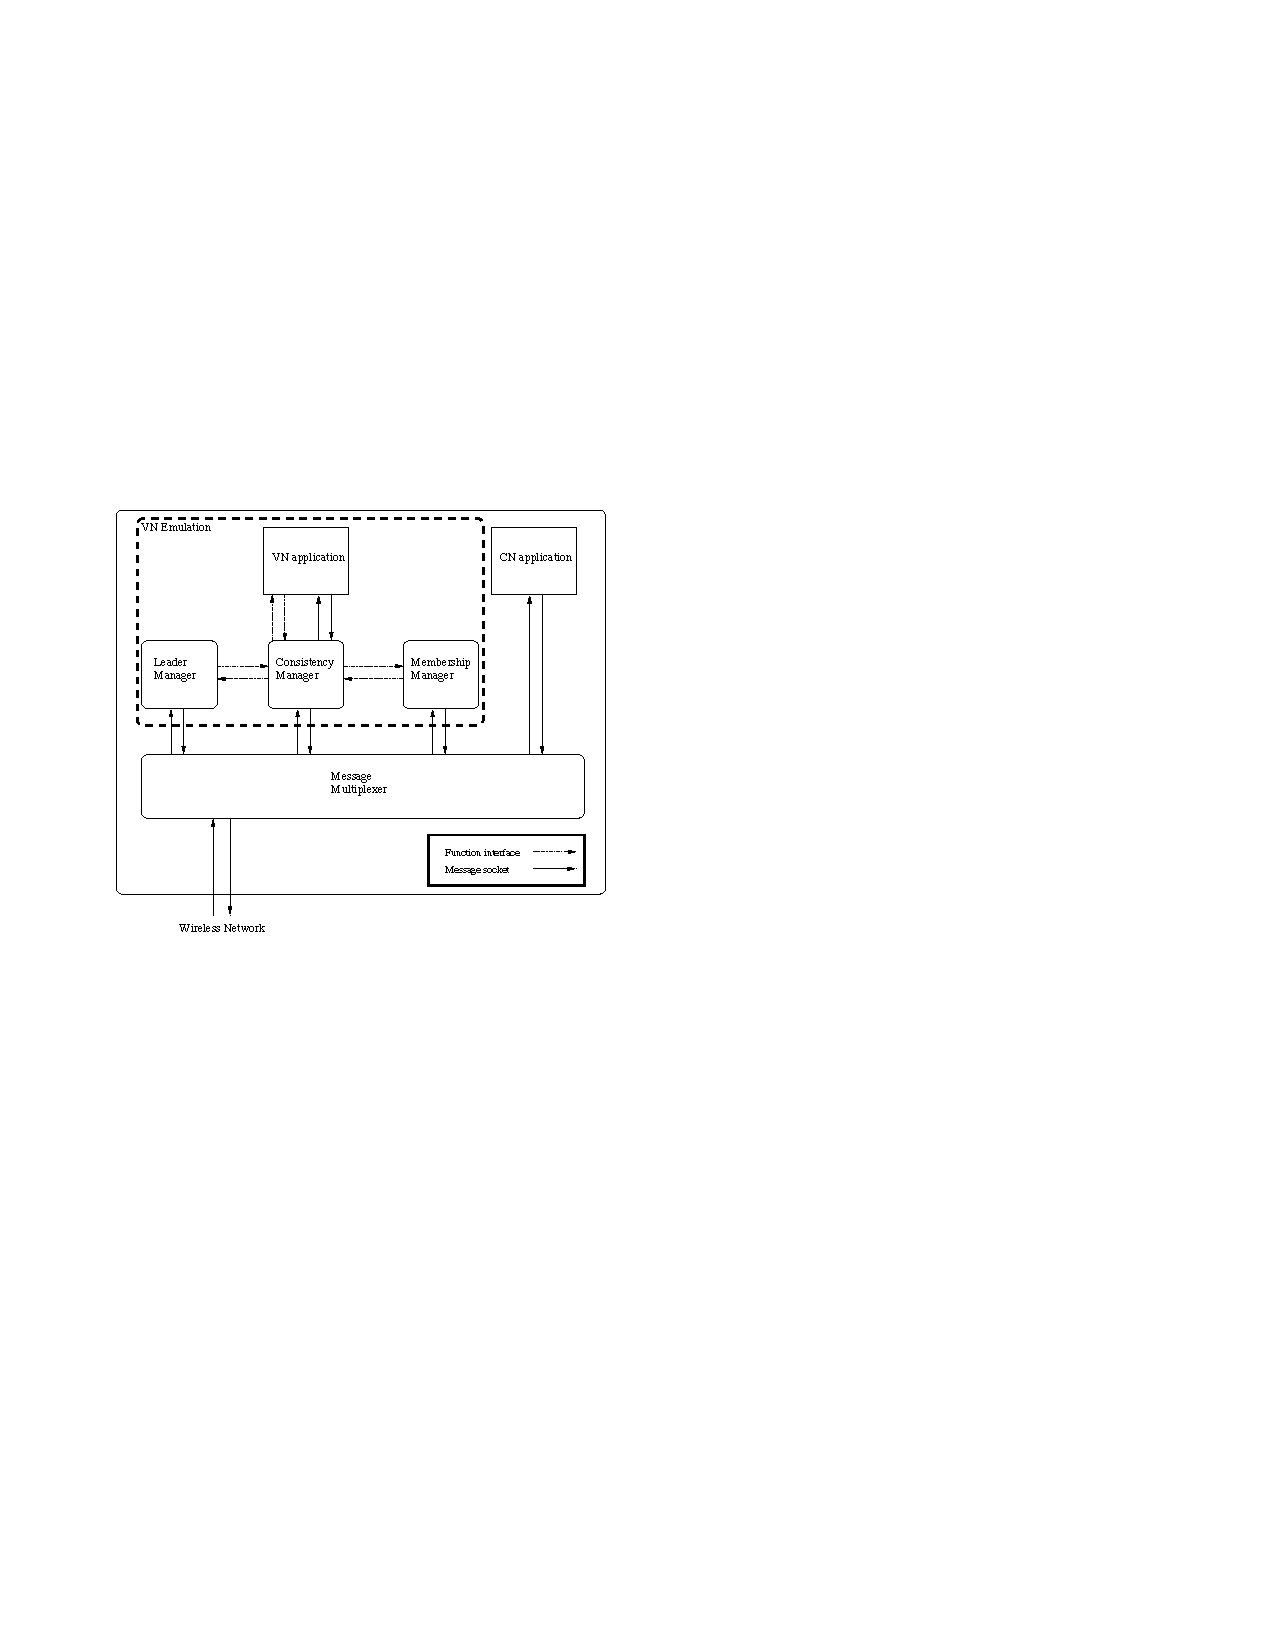
\includegraphics[width=.65\textwidth]{vnlayerarchitecture.pdf} 
\caption{VNLayer Architecture \cite{vnlayer}}
\label{fig:vnlayerArch}
\end{figure}
The VNLayer abstraction is implemented by the client nodes; this means the emulation software must maintain a consistent view of the layer.  In order to do this in a fault tolerant manner, the VN application uses  {\bf leader, consistency, and membership managers} as outlined in figure \ref{fig:vnlayerArch}.  The following is a description of the three managers and VN application:
\begin{description}
\item[Leader Manager:] Elects a leader in the region about the VN and returns  the leader status of the physical node it is running.
\item[Membership Manager:] Returns the current state or a time-out of the emulated VN application.  A time out occurs if there are no other nodes in the region about the VN.
\item[Consistency Manager:] This component is in charge of keeping the emulated VN synchronized with the physical nodes in the region. It calls upon the leadership and membership managers.\\
This component also implements the incoming and outgoing message sockets used in the VN application. 

\item[VN Application:] This implements {\em getState} and {\em updateState} functions that are called by the Consistency Manager.  $getState$ returns the VN applications current state and $updateState$ resets the state to the values passed in as parameter to the function.  
\end{description}

\subsubsection{Reactive VNLayer}
$Reactive\ VNs$ are event-driven automata: their operations occur upon receiving a message which can transform the automata state and potentially return messages to be broadcast in response.  The VNs are located at fixed, known location and fail if the region about the VN does not contain any physical nodes.  In addition, the Reactive VNLayer allows messages to be lost.  
In the Reactive VNLayer, the three managers described above have the following implementation properties: 
\begin{description}
\item[Leader Manager:] This component uses a pulse-based algorithm: the leader sends out a pulse at regular intervals.  If the pulse times out, the client node tries to declare itself as leader.  If multiple nodes are attempting to declare themselves as leader, the node with the lowest ID is selected.  \\
Due to message loss, multiple nodes might elect themselves as leader. This is handled by having any leader who hears a pulse from a  leader with a lower ID relinquish its status as leader.  
\item[Membership Manager:] This uses a simple join protocol, which asks the leader for emulated VN applications state.  If no leader exists, this request times out. 
\item[Consistency Manager:]In the Reactive VNLayer, all physical nodes emulate the VN application, but only the leader broadcasts the VN Application's messages.  
\end{description}
\subsubsection{Virtual Traffic Light}
As outlined in \cite{vnlayer}, the virtual traffic light is a possible application of the Reactive VNlayer.  We assume that each client has access to information about the time and its current location and can communicate with other clients using a local broadcast service. Then, the VN for the intersection is emulated by the CNs that are being run by the physical, autonomous cars approaching and leaving the intersection. 

The VN is programed to inform the CNs approaching the intersection the color of the traffic light in its direction.  To insure progress, the VN keeps track of the amount of time the intersection has shown a certain color.  Although the Reactive VN does not have a clock, the CNs do  (from assumption), and each time a CN sends a message it timestamps it with its clock time.  This is then used by the VN for the best estimated of the current time.   

The algorithm goes as follows:  Clients broadcast their current time, position, and heading in UPDATE messages.  The VNLayer reacts to the message in a $msgReceived$ function as shown in figure \ref{fig:vnlayerAlg}.  The VN for this application is programmed to update its state upon receiving this message and possibly change the color of some of the roads' lights based on the $UpdateLightState$ function. 

\begin{figure}
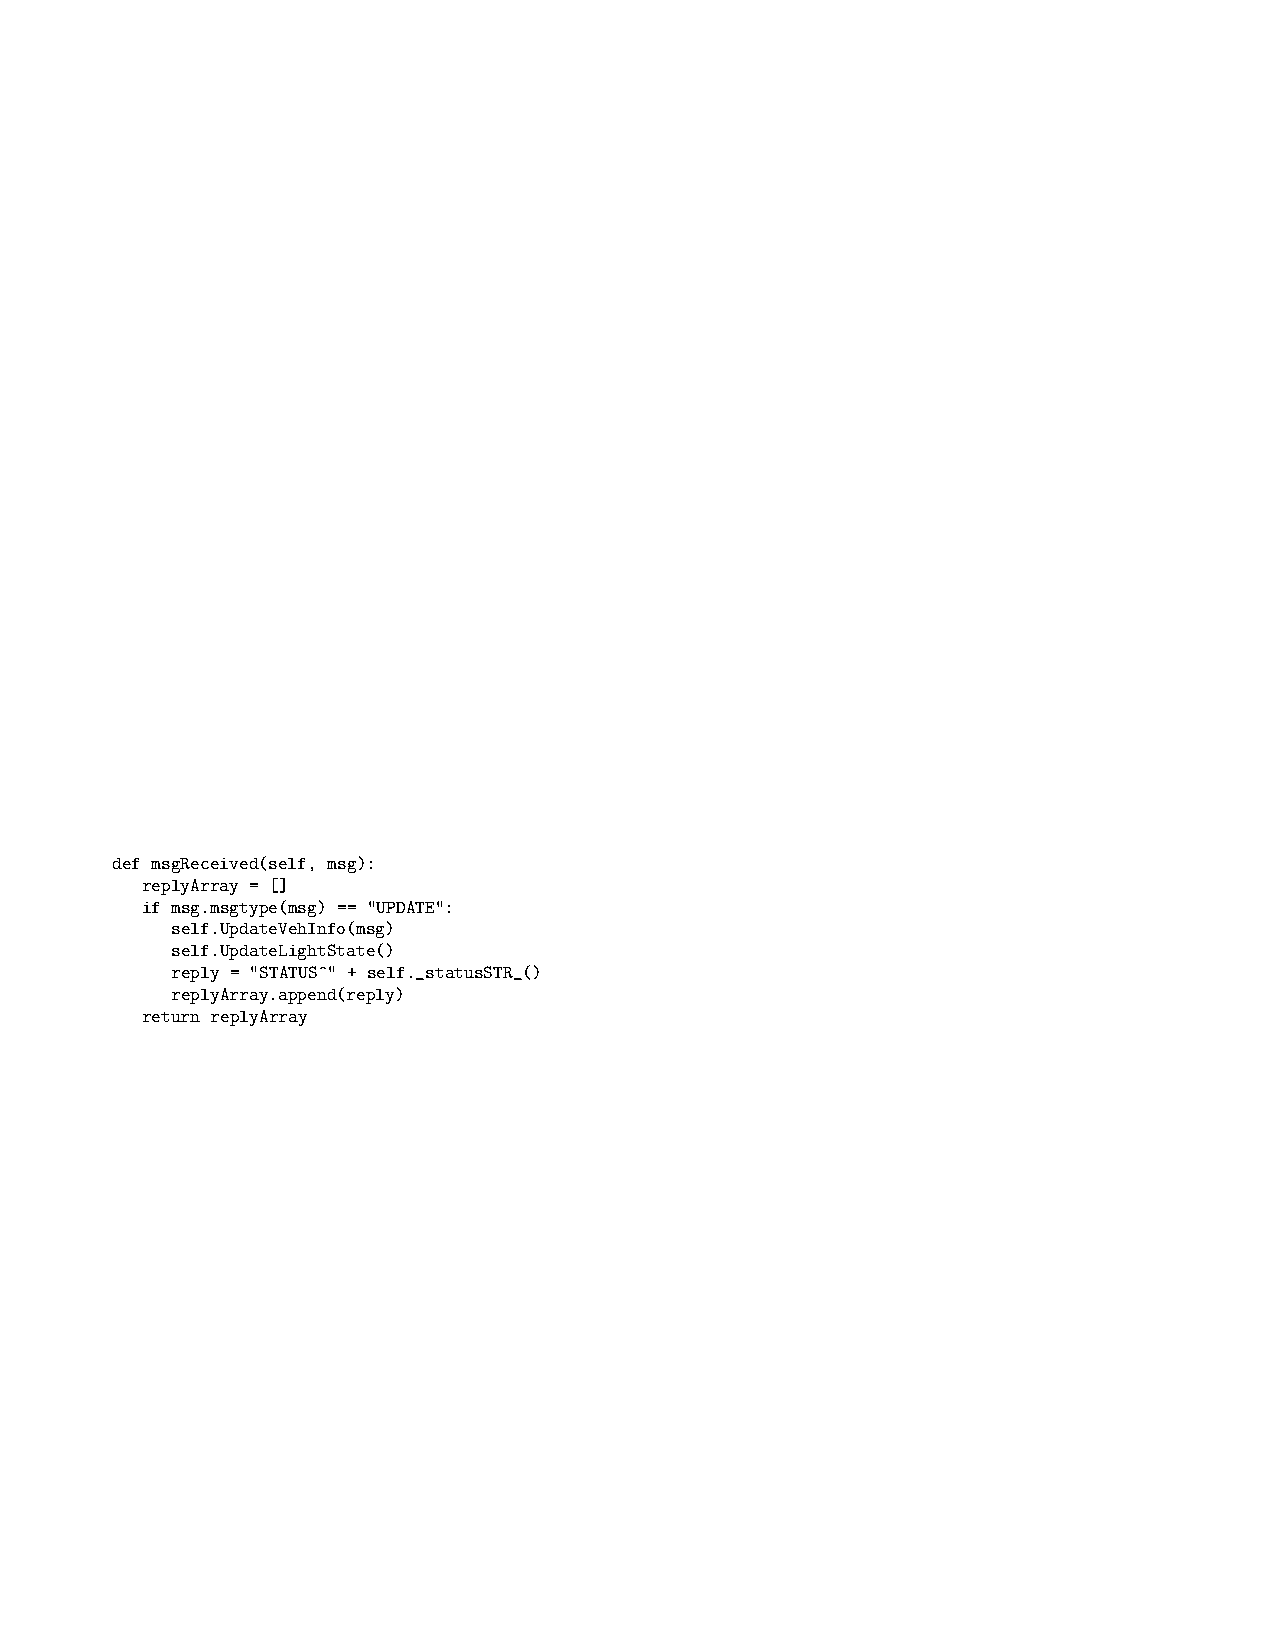
\includegraphics[width=.65\textwidth]{vnlayerAlg.pdf}
\caption{Code for the $msgReceived$ function \cite{vnlayer}}
\label{fig:vnlayerAlg}
\end{figure}
The $UpdateLightFunction$ works as follows: whenever the VN determines that a predetermined minimum "green time" has passed for the green light for a direction , or if it sees that there are no more vehicles heading in that direction, then it changes the direction's lights to yellow.  Then, once the VN sees a predetermined "yellow time" has passed it changes the direction for that light to red and the opposite direction to green.  

\subsection{Liveness and Safety Properties}
\begin{description}
\item[Safety]
 In this implementation, the following safety property is satisfied: only clients in a single direction see a non-red light.
\item[Liveness] 
 Essentially, $UpdateLightState$ works in a round robin fashion, granting green lights to populated direction in order.  This ordering insures the algorithm is fair and cars do not have to wait indefinitely to receive a green light. 
\end{description}

\subsection{Self-Stabilization}
The VNLayer has the self-stabilization property:  the ability to recover from an arbitrarily corrupt state\cite{ssvnlayer}.  Note that in the Leadership manager, the system works by pulsing messages and can elect more than one leader, which eventually gets fixed because the leader with the higher ID will relinquish its status after receiving a message from a leader with a lower ID. 
\subsection{Conclusion}
One concern with this approach is that the behavior of the stop light can be inconsistent until the VNLayer  self-stabilizes. This stoplight might work ideally in a intersection where there are always cars within the network so the VN application is consistently being emulated in a stable configuration. 
Maybe something else? %XXX Could this fail the safety property or just make vehicles wait until stabilization is achieved?
Unlike the algorithms in Section \ref{sec:tokenRing} and \ref{sec:DNF}, the traffic light application for VNLayers does not handle the extra evaluation criteria outlined in \ref{sec:problemDefinition}.  However, the abstraction to VNs and CNs makes the ability to program the application much simpler.  It is possible that messages from CNs could include more information for the $updateLightStatus$ to use.  For example, the message could include a boolean value $isAmbulance$ which the $updateLightStatus$ will use to change the light to the ambulance's direction faster than the predetermined wait time. 

\section{Future Work}
\label{sec:futureWork}
A great deal of research has focused on creating centralized autonomous intersection algorithms; this is probably due to the ease of programming of the application.  Creating a fault tolerant decentralized algorithm is nontrivial;  however, the Reactive VNLayers greatly simplifies this process.  The  centralized virtual traffic light implemented using Reactive VNLayers described in Section \ref{sec:VNLayer} could potentially be extended to implement more advanced centralized autonomous intersection algorithms.  For example, the traffic light application currently does not take into account priority of other vehicles or improving throughput,  fuel consumption, or the amount of time the cars are stopped as described in other algorithms.  However, since VNLayer allows us to emulate a centralized traffic controller, it's possible we could adapt centralized algorithms such as %XXX
to create an approach that is decentralized, but has the desired evaluation properties outlined in Section \ref{sec:problemDefinition}, in addition to the properties of the centralized algorithms it simulates.   %bla this is bad I talked about this in conclusion earlier...



\section{Conclusion}
We have surveyed the intersection management problem, which concerns the behavior of autonomous vehicles at intersections. We have considered it from a distributed point of view, which has the advantage of requiring no new infrastructure spending. It does require new software in all vehicles, but with autonomous vehicles this software will need to be new in any case.\par
We have considered two broad approaches. The first approach was to treat the problem as a distributed problem. We discussed two papers to use this approach. The first was based on ideas from mutual exclusion, where vehicles obtained discrete sections of the intersection. When vehicles controlled their entire path through the intersection, they are allowed to proceed through the intersection, which prevents any crashes from occuring. We also considered an approach which relied directly on motion planning work. There vehicles are free to move in arbitrary diretions, and sense other vehicles to stop from coming too close to them. This takes inspiration from a shared memory model, where vehicles continually update their positions in memory. Though the approach is an interesting one, there are many issues with the assumptions made by the authors of the algorithm that seem to make it unfeasible to use.\par
We also considered an approach that used virtual nodes to emulate a stoplight system. Although we examined the stoplight system in detail, virtual nodes can be used to emulate an arbitrary centralized system. This is very useful for the problem, as most of the research done into intersection management has considered a centralized approach.\par
Both approaches show promise, though the papers that treated the problem directly as a decentralized problem need more formalization. In order for a system to be implemented in reality the problem needs to be studied with assumptions made about transient message failures, as well as a protocol for what to do when stopping failures occur, as rare as they may be. The throughput and fairness of the systems should also be compared to the current systems in use today, such as stoplights and stop signs.

\label{sec:conclusion}

\pagebreak

\begin{thebibliography}{9}

\bibitem{dresner}
Kurt Dresner and Peter Stone. ''Multiagent Traffic Management: An Improved Intersection
Control Mechanism", AAMAS'05 Proceedings of the fourth international joint conference on Autonomous agents and multiagent systems, New York, NY, USA, 2005.
\bibitem{naumann}
Naumann, Rolf, and Rainer Rasche. ``Intersection collision avoidance by means of decentralized security and communication management of autonomous vehicles", Univ.-GH, SFB 376, 1997.
\bibitem{tszchiu}
Au, Tsz-Chiu, Neda Shahidi, and Peter Stone. ``Enforcing Liveness in Autonomous Traffic Management." AAAI. 2011.
\bibitem{roozbehani}
Roozbehani, Hajir, Sylvain Rudaz, and Denis Gillet. "On decentralized navigation schemes for coordination of multi-agent dynamical systems." Systems, Man and Cybernetics, 2009. SMC 2009. IEEE International Conference on. IEEE, 2009.
\bibitem{vnlayer}
Brown, Matthew, et al. "The virtual node layer: a programming abstraction for wireless sensor networks." SIGBED Review 4.3 (2007): 7-12.
\bibitem{ssvnlayer}
Nolte, Tina, and Nancy Lynch. ``Self-stabilization and virtual node layer emulations." Stabilization, Safety, and Security of Distributed Systems. Springer Berlin Heidelberg, 2007. 394-408.
\end{thebibliography}
\end{document}
